\documentclass{article}

\usepackage{graphicx}
\usepackage{amsmath}
\usepackage{siunitx}
\usepackage{xcolor}
\usepackage{tikz}
\usepackage[english,german]{babel}

\definecolor{yucky}{HTML}{dee2e6}
\definecolor{yuckytext}{HTML}{343a40}

\usetikzlibrary{shapes,arrows}

\tikzstyle{decision} = [diamond, draw, fill=blue!20,
    text width=4.5em, text badly centered, node distance=3cm, inner sep=0pt]
\tikzstyle{block} = [rectangle, draw=yucky, fill=yucky, text=yuckytext,
    text width=10em, text centered, rounded corners, minimum height=4em, minimum width=10em]
\tikzstyle{line} = [draw, -latex']
\tikzstyle{cloud} = [draw, ellipse,fill=red!20, node distance=3cm,
    minimum height=2em]

\begin{document}

\begin{center}
\Large{Messtechnikversuch P02: NTC-Thermistor}
\end{center}

\begin{flushright}
  R. Grünert\\
  01.10.2020
\end{flushright}



\section{Auswertung der Messwerte}

\subsection{Statische Kennlinie des NTC}
Die Ermittlung der statischen Kennlinie des Widerstands-/Temperaturverlaufes $R=f(T)$ des NTC Thermistors vom Hersteller Vishay konnte aus den im Datenblatt angegebenen Parametern und der \textit{Steinhart-and-Hart-Gleichung} ermittelt werden.\\

Der NTC besitzt den Farbcode \textit{I: Orange, II: Orange, III: Orange, IV: Gold} und hat somit die Kennwerte
\[R_{25} = 33000 \, \si{\ohm} \pm 5 \, \si{\percent}\]
\[B_{25/85} = 4090 \, \si{\kelvin} \pm 1.5 \, \si{\percent}\]

Aus dem Datenblatt:
\[
  R_{T/K} = R_{25} \cdot e^{(A + B/T + C/T^{2} + D/T^{3})},
\]
\begin{align*}
  \text{mit}~A &= -15.5322, \\
  B &= 5229.973 \, \si{\kelvin}\\
  C &= -160451 \, \si{\kelvin}^{2}\\
  D &= -5.414091 \cdot 10^{6} \, \si{\kelvin}^{3}
\end{align*}

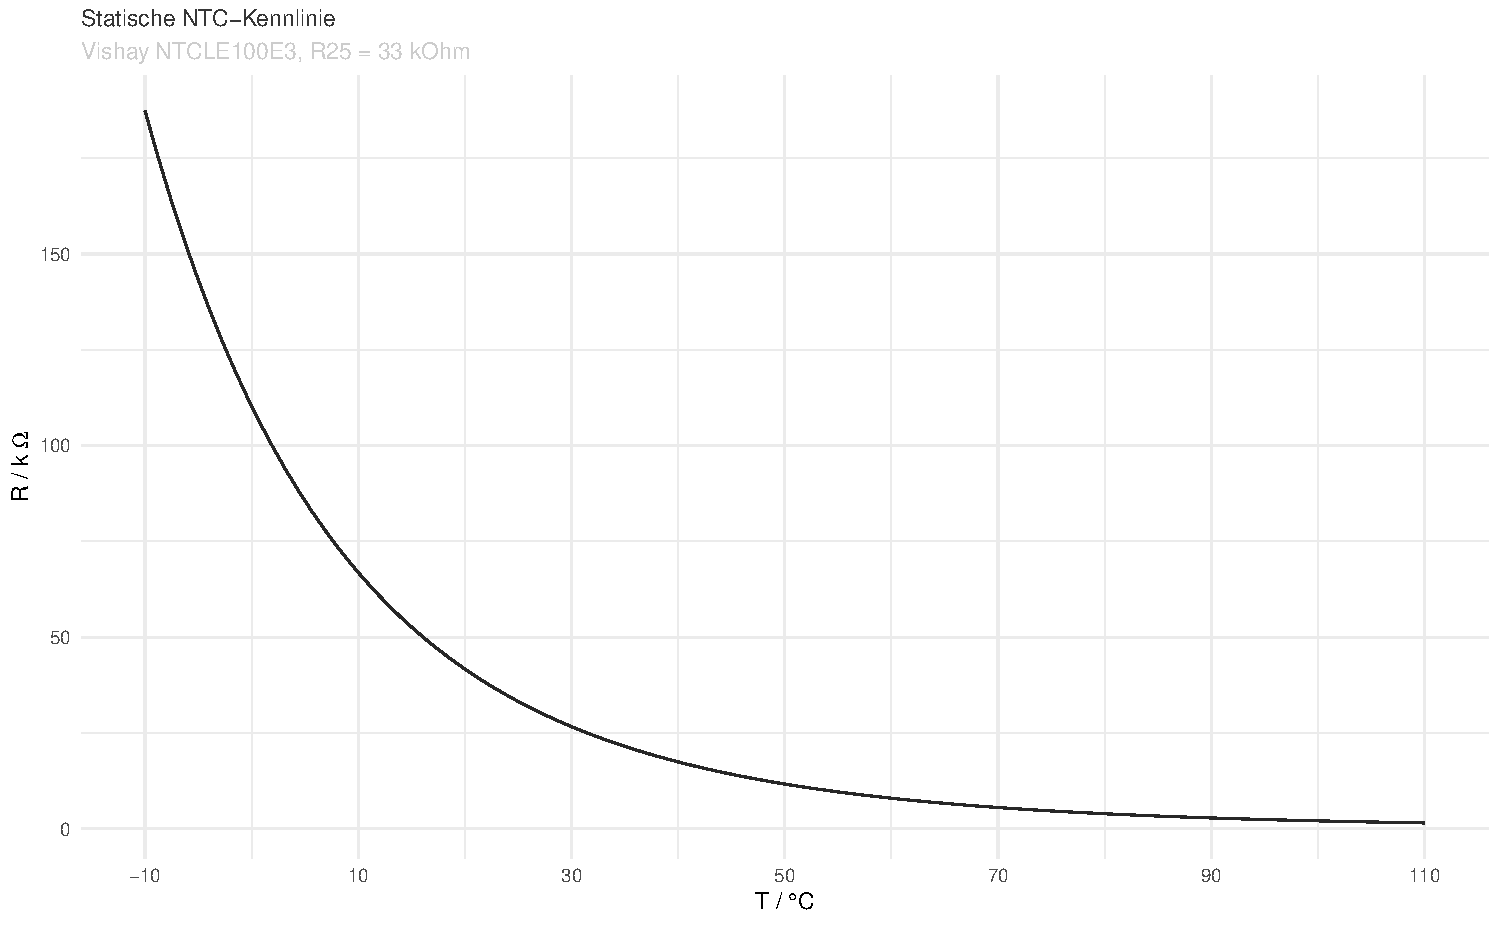
\includegraphics[width=\textwidth]{graphics/ntcStatischeKennlinie.pdf}

\end{document}
